% [R01]
\subsection{Motivating Example}
\label{sec:motivating-example}

% [R02]
Figure~\ref{fig:motivating-example} presents a message-processing
example that illustrates the need to track type-state changes across
function calls. The function \texttt{make\_line} calls
\texttt{encode\_message} to encode a message body before appending
a newline. The body is declared as \texttt{str | bytes}.
For a string body, \texttt{encode\_message} invokes the supplied
encoder and stores its result in the same message object.
\texttt{TextEncoder} returns the string unchanged, whereas
\texttt{Utf8Encoder} converts it to bytes.

% [R02a]
As shown in the figure, Mypy, Pyrefly, and Pyright do not report the
concatenation error, whereas PyTT detects it. Analyzing this example
reveals two related requirements for type-error detection. First,
the analyzer must propagate changes to the shared message body across
the call so that the subsequent operation is checked against its
updated type. Second, distinguishing the failing UTF-8 call from the
safe text-encoder call requires retaining the conditions under which
each update occurs. We examine these requirements below and explain
how PyTT addresses them through conditional type-state summaries.

\begin{figure}[!htbp]
\centering
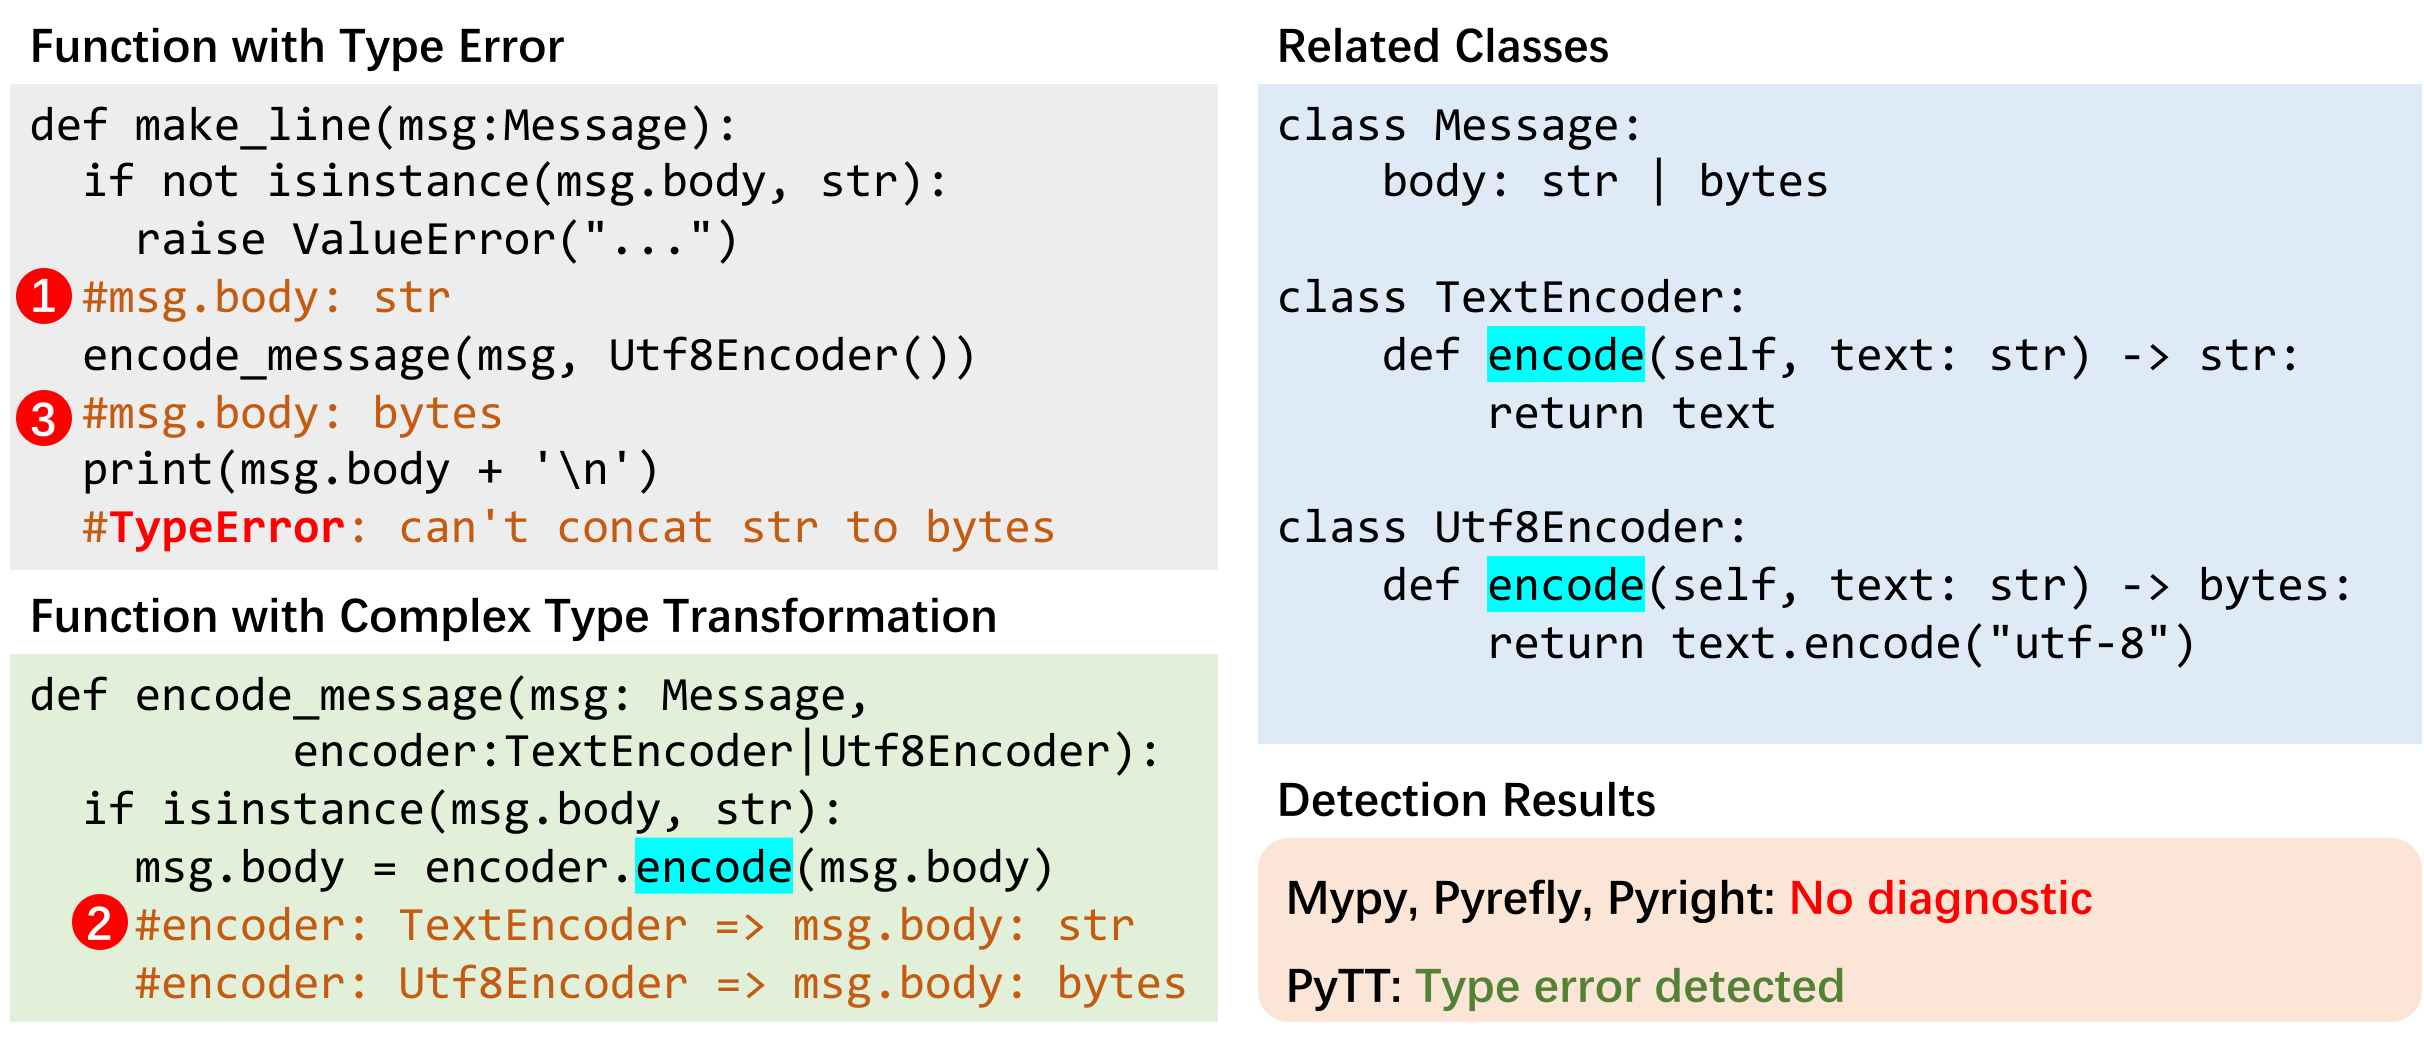
\includegraphics[width=\linewidth]{photos/motivatingExample.png}
% [R03]
\caption{Motivating example of interprocedural type-state changes
and type-error detection results.}
\Description{The caller make_line rejects a non-string message body,
then calls encode_message with Utf8Encoder and attempts to concatenate
msg.body with a newline string. For a string input, the helper writes
the encoder's result into the same message object. TextEncoder returns
a string, and Utf8Encoder returns bytes. Points 1, 2, and 3 mark the
string body before the call, the conditional field updates, and the
bytes body after the UTF-8 call returns normally. The concatenation
then raises TypeError. The result panel labels Mypy, Pyrefly, and
Pyright with No diagnostic and PyTT with Type error detected.}
\label{fig:motivating-example}
\end{figure}

% [R04]
\textbf{(1) Interprocedural Type-State Propagation.}
In \texttt{make\_line}, the guard raises \texttt{ValueError} when
\texttt{msg.body} is not a string. Thus, the body has type
\texttt{str} at point~1. The subsequent call passes \texttt{msg}
and a \texttt{Utf8Encoder} instance to \texttt{encode\_message},
which writes the encoding result into \texttt{msg.body}. Because
both functions access the same message object, the body has type
\texttt{bytes} at point~3 after the call returns normally.
The expression \texttt{msg.body + '\textbackslash n'} then raises
\texttt{TypeError} before \texttt{print} is invoked, and the exception
escapes \texttt{make\_line}.

% [R05]
Both the original string and the updated bytes satisfy the field's
union annotation, but the updated body does not support concatenation
with a string. Detecting this error requires propagating the field
update from \texttt{encode\_message} to its caller. The function's
return type, \texttt{None}, does not describe this update. If the
analyzer retains the string type established at point~1, it can miss
the error at point~3.

% [R06]
\textbf{(2) Conditional Type-State Modeling.}
Propagating a field update also requires determining which type the
call establishes. In this example, that type depends on the encoder
argument. Replacing \texttt{Utf8Encoder} with
\texttt{TextEncoder} leaves a string body and makes the concatenation
valid. An analyzer that assigns \texttt{str | bytes} to the body
after either call can flag the potential bytes/string conflict.
However, retaining the bytes alternative for \texttt{TextEncoder}
can also cause a false alarm. Distinguishing these calls therefore
requires preserving the relation between the encoder argument and the
resulting field type under the incoming string condition.

% [R07]
PyTT addresses these requirements using path-sensitive type contracts
(PSTCs), which record field updates together with their calling
conditions and propagate the applicable updates to callers. At point~2,
the contract for \texttt{encode\_message} records two cases for an
incoming string body. On normal return, the \texttt{TextEncoder}
case establishes a string body, and the \texttt{Utf8Encoder} case
establishes a bytes body. For a non-string input, the function leaves
the body unchanged.

% [R08]
At the illustrated call, PyTT uses the string type established by the
guard and the \texttt{Utf8Encoder} argument to select the second case.
It maps the callee's message parameter to the caller's object and
updates the type of \texttt{msg.body} accordingly. The subsequent
concatenation is therefore checked with a bytes body, revealing the
type error.
